\chapter{Specifikacija programske potpore}
		
	\section{Funkcionalni zahtjevi}
			
			\noindent \textbf{Dionici:}
			
			\begin{packed_enum}
				
				\item Direktor službe
				\item Korisnici stranice
				
				\begin{packed_enum}
				
						\item Neregistrirani korisnici
						\item Registrirani korisnici
						
				\end{packed_enum}
				
				\item Službenici	
				\item Razvojni tim	
				
				
			\end{packed_enum}
			
			\noindent \textbf{Aktori i njihovi funkcionalni zahtjevi:}
			
			
			\begin{packed_enum}
				\item  \underbar{Neregistrirani/neprijavljeni korisnik (inicijator) može:}
				
				\begin{packed_enum}
					
					\item na karti pregledati pozicije kontejnera
					\item pronaći kontejner pomoću njegovog ID-a ili adrese
					\item vidjeti trenutno i stanje kontejnera do 3 mjeseca unatrag
					\item registrirati se u sustav te stvoriti novi korisnički račun za koji su mu potrebni korisničko ime, lozinka i e-mail adresa
					
				\end{packed_enum}
			
				\item  \underbar{Registrirani korisnik (inicijator) može:}
				
				\begin{packed_enum}
					
					\item pregledavati i mijenjati svoje osobne podatke
					\item izbrisati svoj korisnički račun
					\item ocijeniti stanje i pisati komentare o kontejneru
					\item postaviti fotografije kontejnera
					\item odabrati kontejnere za praćenje njihovog stanja
					
				\end{packed_enum}
				
					\item \underbar{Službenik (inicijator) može:}
				
				\begin{packed_enum}
				
					\item označiti da je ispraznio kontejner 
					\item premjestiti kontejner
					\item povući kontejner u skladište
				
				\end{packed_enum}	
				
				\item \underbar{Direktor službe (inicijator) može:}		
				
				\begin{packed_enum}
				
					\item dodati i izbrisati korisnika iz svoje službe
					\item dodati, izbrisati i premjestiti kontejner 				
				
				\end{packed_enum}
				
				\item	\underbar{Baza podataka (sudionik):}
				
				\begin{packed_enum}
				
					\item pohranjuje sve podatke o korisnicima i njihovim ovlastima
					\item pohranjuje sve podatke o kontejnerima 
				
				\end{packed_enum}
				
			\end{packed_enum}
			
			\eject 
			
			
				
			\subsection{Obrasci uporabe}
			
			\textbf{\textit{dio 1. revizije}}
			
			\subsubsection{Opis obrazaca uporabe}
			
			\noindent \underbar{\textbf{UC1 - Pretraživanje i pregled kontejnera putem ID-a}}
			\begin{packed_item}
				
				\item \textbf{Glavni sudionik:} Svi korisnici
				\item  \textbf{Cilj:} Pregledati kontejnere i njihovo stanje kroz vremenski period
				\item  \textbf{Sudionici:} Baza podataka
				\item  \textbf{Preduvjet:} -
				\item  \textbf{Opis osnovnog tijeka:}
				
				\item[] \begin{packed_enum}
					
					\item Korisnik u tražilicu upisuje ID kontejnera
					\item Prikazuju se informacije o kontejneru
					
				\end{packed_enum}
				
				\item  \textbf{Opis mogućih odstupanja:}
				
				\item[] \begin{packed_item}
					
					\item[2.a] Neispravan/nepostojeći ID
					\item[] \begin{packed_enum}
						
						\item Sustav obavještava korisnike o neuspjelom pokušaju te navodi korisnika na upis valjanog ID-a
						\item Korisnik upisuje ispravan ID ili odustaje od pretraživanja
					\end{packed_enum}
					
				\end{packed_item}
			\end{packed_item}
			
			\noindent \underbar{\textbf{UC2 - Pretraživanje i pregled kontejnera odabirom na karti/putem adrese}}
			\begin{packed_item}
				
				\item \textbf{Glavni sudionik:} Svi korisnici
				\item  \textbf{Cilj:} Pregledati kontejnere i njihovo stanje kroz vremenski period 
				\item  \textbf{Sudionici:} Baza podataka
				\item  \textbf{Preduvjet:} -
				\item  \textbf{Opis osnovnog tijeka:}
				
				\item[] \begin{packed_enum}
					
					\item Karta je prikazana prilikom učitavanja aplikacije
					\item Korisnik na karti odabire kontejner 
					\item Prikazuju se informacije o kontejneru 
					
				\end{packed_enum}
			\end{packed_item}
			
			
			\noindent \underbar{\textbf{UC3 - Registracija}}
			\begin{packed_item}
				
				\item \textbf{Glavni sudionik:} Neregistrirani korisnici
				\item  \textbf{Cilj:} Stvoriti korisnički račun za pristup sustavu
				\item  \textbf{Sudionici:} Baza podataka
				\item  \textbf{Preduvjet:} -
				\item  \textbf{Opis osnovnog tijeka:}
				
				\item[] \begin{packed_enum}
					
					\item Korisnik odabire opciju za registraciju
					\item Korisnik unosi potrebne korisničke podatke 
					\item Korisnik prima obavijest o uspješnoj registraciji
					
				\end{packed_enum}
				
				\item  \textbf{Opis mogućih odstupanja:}
				
				\item[] \begin{packed_item}
					
					\item[3.a] Odabir vec zauzetog korisničkog imena i/ili e-maila, unos korisničkog podatka u nedozvoljenom formatu ili pružanje neispravnoga e-maila 
					\item[] \begin{packed_enum}
						
						\item Sustav obavještava korisnika o neuspjelom upisu i vraća ga na stranicu za registraciju
						\item Korisnik mijenja potrebne podatke te završava unos ili odustaje od registracije
					\end{packed_enum}
					
				\end{packed_item}
			\end{packed_item}
			
			
			\noindent\underbar{\textbf{UC4 - Prijava u sustav}}
			\begin{packed_item}
				
				\item \textbf{Glavni sudionik:} Registrirani korisnici, zaposlenici, direktor
				\item  \textbf{Cilj:} Dobiti pristup korisničkom sučelju
				\item  \textbf{Sudionici:} Baza podataka
				\item  \textbf{Preduvjet:} Registracija
				\item  \textbf{Opis osnovnog tijeka:}
				
				\item[] \begin{packed_enum}
					
					\item Unos korisničkog imena i lozinke
					\item Potvrda o ispravnosti unesenih podataka
					\item Pristup funkcijama
					
				\end{packed_enum}
				
				\item  \textbf{Opis mogućih odstupanja:}
				
				\item[] \begin{packed_item}
					
					\item[2.a] Neispravno korisničko ime/lozinka
					\item[] \begin{packed_enum}
						
						\item Sustav obavještava korisnike o neuspješnom upisu 
						\item Korisnik upisuje ispravne podatke ili odustaje od prijave
					\end{packed_enum}
					
				\end{packed_item}
			\end{packed_item}
			
			\noindent \underbar{\textbf{UC5 - Pregled osobnih podataka}}
			\begin{packed_item}
				
				\item \textbf{Glavni sudionik:} Registrirani korisnici, zaposlenici, direktor
				\item  \textbf{Cilj:} Pregledati osobne podatke
				\item  \textbf{Sudionici:} Baza podataka
				\item  \textbf{Preduvjet:} Klijent je prijavljen
				\item  \textbf{Opis osnovnog tijeka:}
				
				\item[] \begin{packed_enum}
					
					\item Korisnik odabire opciju "Osobni podatci"
					\item Prikazuju se osobni podatci korisnika
					
				\end{packed_enum}
			\end{packed_item}
			
			\noindent \underbar{\textbf{UC6 - Objava slike kontejnera}}
			\begin{packed_item}
				
				\item \textbf{Glavni sudionik:} Registrirani korisnik
				\item  \textbf{Cilj:} Objaviti trenutno stanje kontejnera
				\item  \textbf{Sudionici:} Baza podataka
				\item  \textbf{Preduvjet:} Korisnik je prijavljen
				\item  \textbf{Opis osnovnog tijeka:}
				
				\item[] \begin{packed_enum}
					
					\item Korisnik odabere kontejner
					\item Korisnik učitava sliku kontejnera
					\item Korisnik objavljuje sliku kontejnera
					
				\end{packed_enum}
				
				\item  \textbf{Opis mogućih odstupanja:}
				
				\item[] \begin{packed_item}
					
					\item[2.a] Korisnik učita sliku, ali ju ne objavi
					\item[] \begin{packed_enum}
						
						\item Sustav obavještava korisnika da slika nije objavljena prije obustavljanja radnje
						
					\end{packed_enum}
					
				\end{packed_item}
			\end{packed_item}
			
			\noindent \underbar{\textbf{UC7 - Ocjenjivanje kontejnera}}
			\begin{packed_item}
				
				\item \textbf{Glavni sudionik:} Registrirani korisnik
				\item  \textbf{Cilj:} Ocijeniti trenutno stanje kontejnera
				\item  \textbf{Sudionici:} Baza podataka
				\item  \textbf{Preduvjet:} Korisnik je prijavljen
				\item  \textbf{Opis osnovnog tijeka:}
				
				\item[] \begin{packed_enum}
					
					\item Korisnik odabere kontejner
					\item Korisnik daje ocjenu kontejneru
					
				\end{packed_enum}
			\end{packed_item}
			
			\noindent \underbar{\textbf{UC8 - Komentiranje kontejnera}}
			\begin{packed_item}
				
				\item \textbf{Glavni sudionik:} Registrirani korisnik
				\item  \textbf{Cilj:} Komentirati stanje kontejnera
				\item  \textbf{Sudionici:} Baza podataka
				\item  \textbf{Preduvjet:} Korisnik je prijavljen
				\item  \textbf{Opis osnovnog tijeka:}
				
				\item[] \begin{packed_enum}
					
					\item Korisnik odabere kontejner
					\item Korisnik piše komentar
					\item Korisnik objavljuje komentar
					
				\end{packed_enum}
				
				\item  \textbf{Opis mogućih odstupanja:}
				
				\item[] \begin{packed_item}
					
					\item[2.a] Korisnik napiše komentar, ali ga ne objavi
					\item[] \begin{packed_enum}
						
						\item Sustav obavještava korisnika da komentar nije objavljen prije obustavljanja radnje
						
					\end{packed_enum}
					
				\end{packed_item}
			\end{packed_item}
			
			\noindent \underbar{\textbf{UC9 - Dodavanje  korisnika}}
			\begin{packed_item}
				
				\item \textbf{Glavni sudionik: } Direktor
				\item  \textbf{Cilj:} Dodati novog korisnika
				\item  \textbf{Sudionici:} Baza podataka
				\item  \textbf{Preduvjet:} Direktor mora biti prijavljen
				\item  \textbf{Opis osnovnog tijeka:}
				
				\item[] \begin{packed_enum}
					
					\item Direktor ide na aplikaciju i odabire opciju: dodaj novog korisnika
					\item Direktor upisuje ime, prezime, ID novog korisnika (i ostale podatke koji idu u bazu podataka)
					\item Direktor potvrđuje svoj unos
				\end{packed_enum}
				\item[] \begin{packed_item}

					\item[2.a] Korisnik već postoji u bazi
					\item[] \begin{packed_enum}
						
						\item Sustav izvještava direktora o tome da već postoji korisnik s tim ID-om
						
					\end{packed_enum}
					
				\end{packed_item}
			\end{packed_item}
							
								
			\noindent \underbar{\textbf{UC10 - Brisanje  korisnika}}
			\begin{packed_item}
				
				\item \textbf{Glavni sudionik: } Direktor
				\item  \textbf{Cilj:} Izbrisati postojećeg korisnika
				\item  \textbf{Sudionici:} Baza podataka
				\item  \textbf{Preduvjet:} Direktor mora biti prijavljen
				\item  \textbf{Opis osnovnog tijeka:}
				
				\item[] \begin{packed_enum}
					
					\item Direktor ide na aplikaciju i pretražuje korisnike
					\item Direktor odabire opciju brisanja korisnika
					\item Direktor potvrđuje svoj izbor
				\end{packed_enum}
				
				\item  \textbf{Opis mogućih odstupanja:}
				
				\item[] \begin{packed_item}
					
					\item[2.a] ID korisnika ne postoji u bazi
					\item[] \begin{packed_enum}
						
						\item Ispisati poruku da taj korisnik nije pronađen
						
					\end{packed_enum}
					
				\end{packed_item}
			\end{packed_item}
			
			\noindent \underbar{\textbf{UC11 - Dodavanje  kontejnera}}
			\begin{packed_item}
				
				\item \textbf{Glavni sudionik: } Direktor
				\item  \textbf{Cilj:} Dodati novi kontejner
				\item  \textbf{Sudionici:} Baza podataka
				\item  \textbf{Preduvjet:} Direktor mora biti prijavljen
				\item  \textbf{Opis osnovnog tijeka:}
				
				\item[] \begin{packed_enum}
					
					\item Direktor ide na aplikaciju i odabire opciju: dodaj novi kontejner
					\item Direktor upisuje adresu i ID novog kontejnera 
					\item Direktor potvrđuje svoj unos
				\end{packed_enum}
				
				\item  \textbf{Opis mogućih odstupanja:}
				
				\item[] \begin{packed_item}
					
					\item[2.a] Na odabranoj adresi već postoji kontejner
					\item[] \begin{packed_enum}
						
						\item Pitati direktora želi li postaviti još jedan kontejner na tu adresu
						\item Direktor odabire opciju da ili ne
						
					\end{packed_enum}
					\item[2.b] Već postoji kontejner s tim ID-om
					\item[] \begin{packed_enum}
						
						\item Ispisati poruku da već postoji kontejner s tim ID-om
						
					\end{packed_enum}
					
				\end{packed_item}
			\end{packed_item}
			
			\noindent \underbar{\textbf{UC12 - Brisanje  kontejnera}}
			\begin{packed_item}
				
				\item \textbf{Glavni sudionik: } Direktor
				\item  \textbf{Cilj:} Dodati novog korisnika
				\item  \textbf{Sudionici:} Baza podataka
				\item  \textbf{Preduvjet:} Direktor mora biti prijavljen
				\item  \textbf{Opis osnovnog tijeka:}
				
				\item[] \begin{packed_enum}
					
					\item Direktor ide na aplikaciju pretražuje kontejner po ID-u ili adresi i odabire opciju za brisanje kontejnera
					\item Direktor potvrđuje svoj unos
				\end{packed_enum}
				
				\item  \textbf{Opis mogućih odstupanja:}
				
				\item[] \begin{packed_item}
					
					\item[2.a] Traženi ID kontejnera ne postoji
					\item[] \begin{packed_enum}
						
						\item Ispisati poruku da traženi kontejner nije pronađen
						
					\end{packed_enum}
					\item[2.b] Na traženoj adresi nema niti jednog kontejnera
							\item[] \begin{packed_enum}
						
						\item Ispisati da na traženoj adresi nema niti jednog kontejnera
						
					\end{packed_enum}
					
				\end{packed_item}
			\end{packed_item}
			
			\noindent \underbar{\textbf{UC13 - Premještanje  kontejnera}}
			\begin{packed_item}
				
				\item \textbf{Glavni sudionik: } Direktor
				\item  \textbf{Cilj:} Premjestiti kontejner s jedne lokacije na drugu
				\item  \textbf{Sudionici:} Baza podataka
				\item  \textbf{Preduvjet:} Direktor mora biti prijavljen
				\item  \textbf{Opis osnovnog tijeka:}
				
				\item[] \begin{packed_enum}
					
					\item Direktor ide na aplikaciju i pretražuje kontejner po ID-u ili adresi i odabire opciju za premještanje kontejnera
					\item Direktor upisuje adresu gdje želi da kontejner bude premješten
					\item Direktor potvrđuje svoj unos
				\end{packed_enum}
				
				\item  \textbf{Opis mogućih odstupanja:}
				
				\item[] \begin{packed_item}
					
							\item[2.a] Traženi ID kontejnera ne postoji
					\item[] \begin{packed_enum}
						
						\item Ispisati poruku da traženi kontejner nije pronađen
						
					\end{packed_enum}
					\item[2.b] Na traženoj adresi nema niti jednog kontejnera
					\item[] \begin{packed_enum}
						
						\item Ispisati da na traženoj adresi nema niti jednog kontejnera
							\end{packed_enum}
					\item[2.c] Na odabranoj adresi već postoji kontejner
			
						\item[] \begin{packed_enum}
							
							\item Pitati direktora želi li postaviti još jedan kontejner na tu adresu
							\item Direktor odabire opciju da ili ne
							
						\end{packed_enum}
						
					
				\end{packed_item}
			\end{packed_item}
			
			\noindent \underbar{\textbf{UC14 - Pregled rute}}
			\begin{packed_item}
				
				\item \textbf{Glavni sudionik:} Zaoslenici
				\item  \textbf{Cilj:} Pregledati rutu uz prikazivanje vih kontejnera
				\item  \textbf{Sudionici:} Baza podataka
				\item  \textbf{Preduvjet:} Zaposlenik mora biti prijavljen
				\item  \textbf{Opis osnovnog tijeka:}
				
				\item[] \begin{packed_enum}
					
					\item Zaposlenik pritisne na gumb moja ruta
					\item Prikazuju mu se informacije ruti zaposlenika
					
				\end{packed_enum}
				
				\item  \textbf{Opis mogućih odstupanja:}
				
				\item[] \begin{packed_item}
					
					\item[2.a] Neispravana/nepostojeća ruta
					\item[] \begin{packed_enum}
						
						\item Sustav obavještava zaposlenika o nepostojećoj ruti

					\end{packed_enum}
					
				\end{packed_item}
			\end{packed_item}
			

			\subsubsection{Dijagrami obrazaca uporabe}
            
            \begin{figure}
                    \centering
                    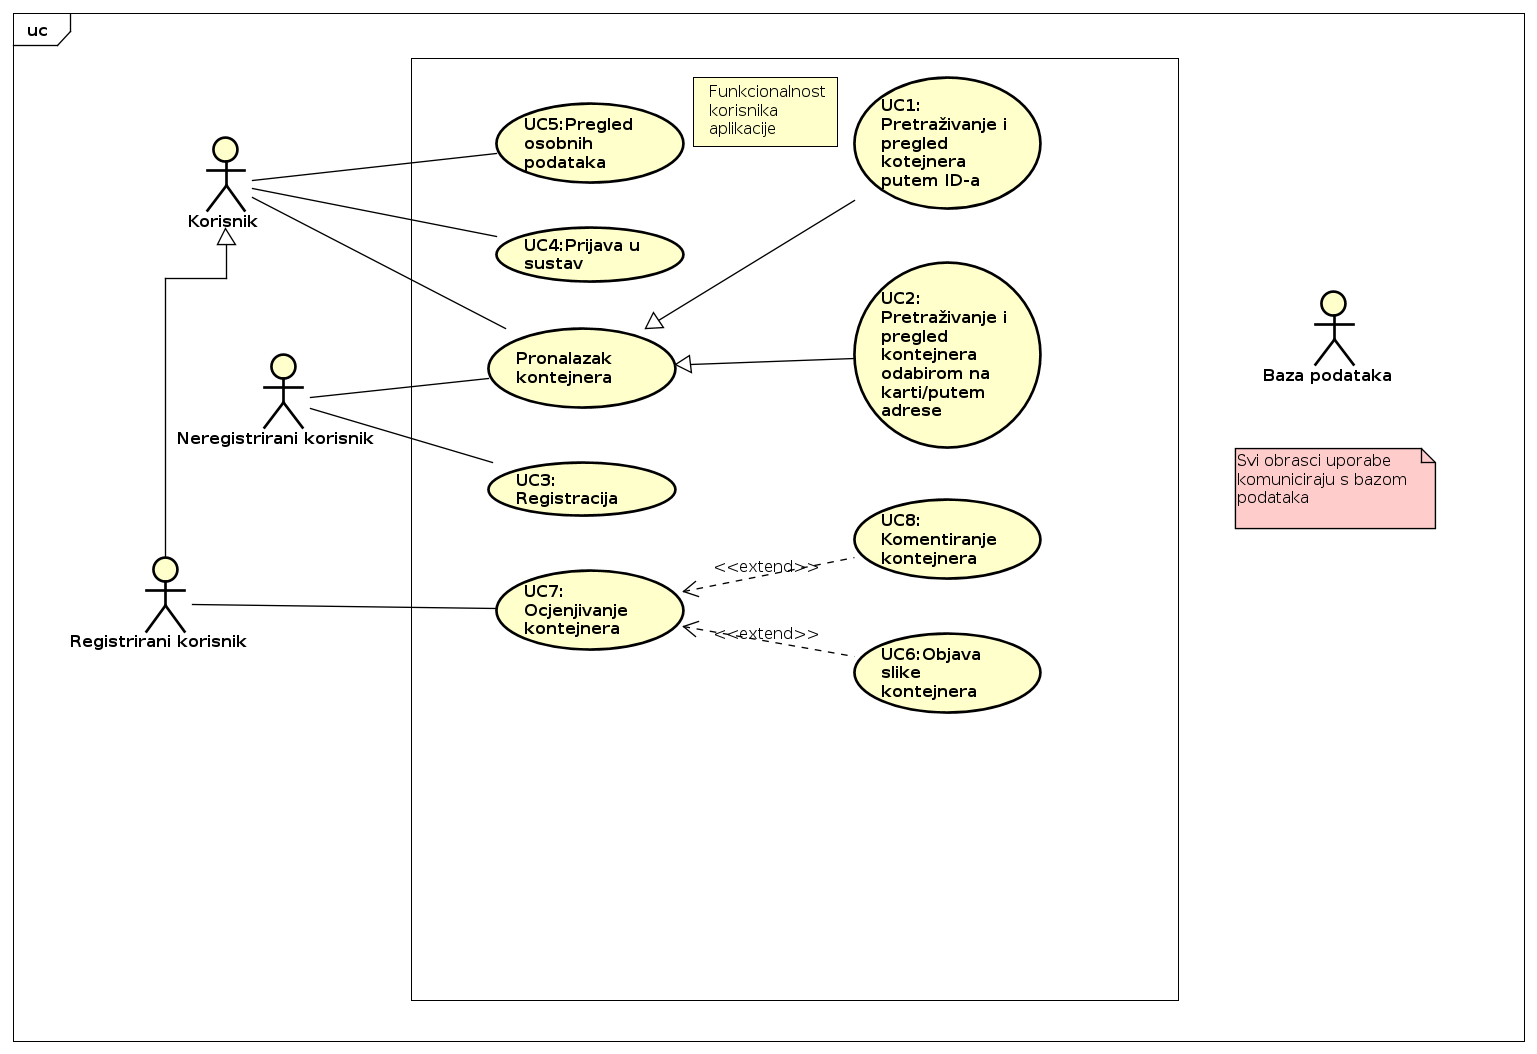
\includegraphics[width=1.0\linewidth]{slike/Funkcionalnost_korisnika_aplikacije.png}
                    \caption{Dijagram obrazaca uporabe, funkcionalnost korisnika aplikacije}
                    \label{fig:Funkcionalnost korisnika aplikacije}
            \end{figure}
            
            \clearpage
            
            \eject
            
            \begin{figure}
                    \centering
                    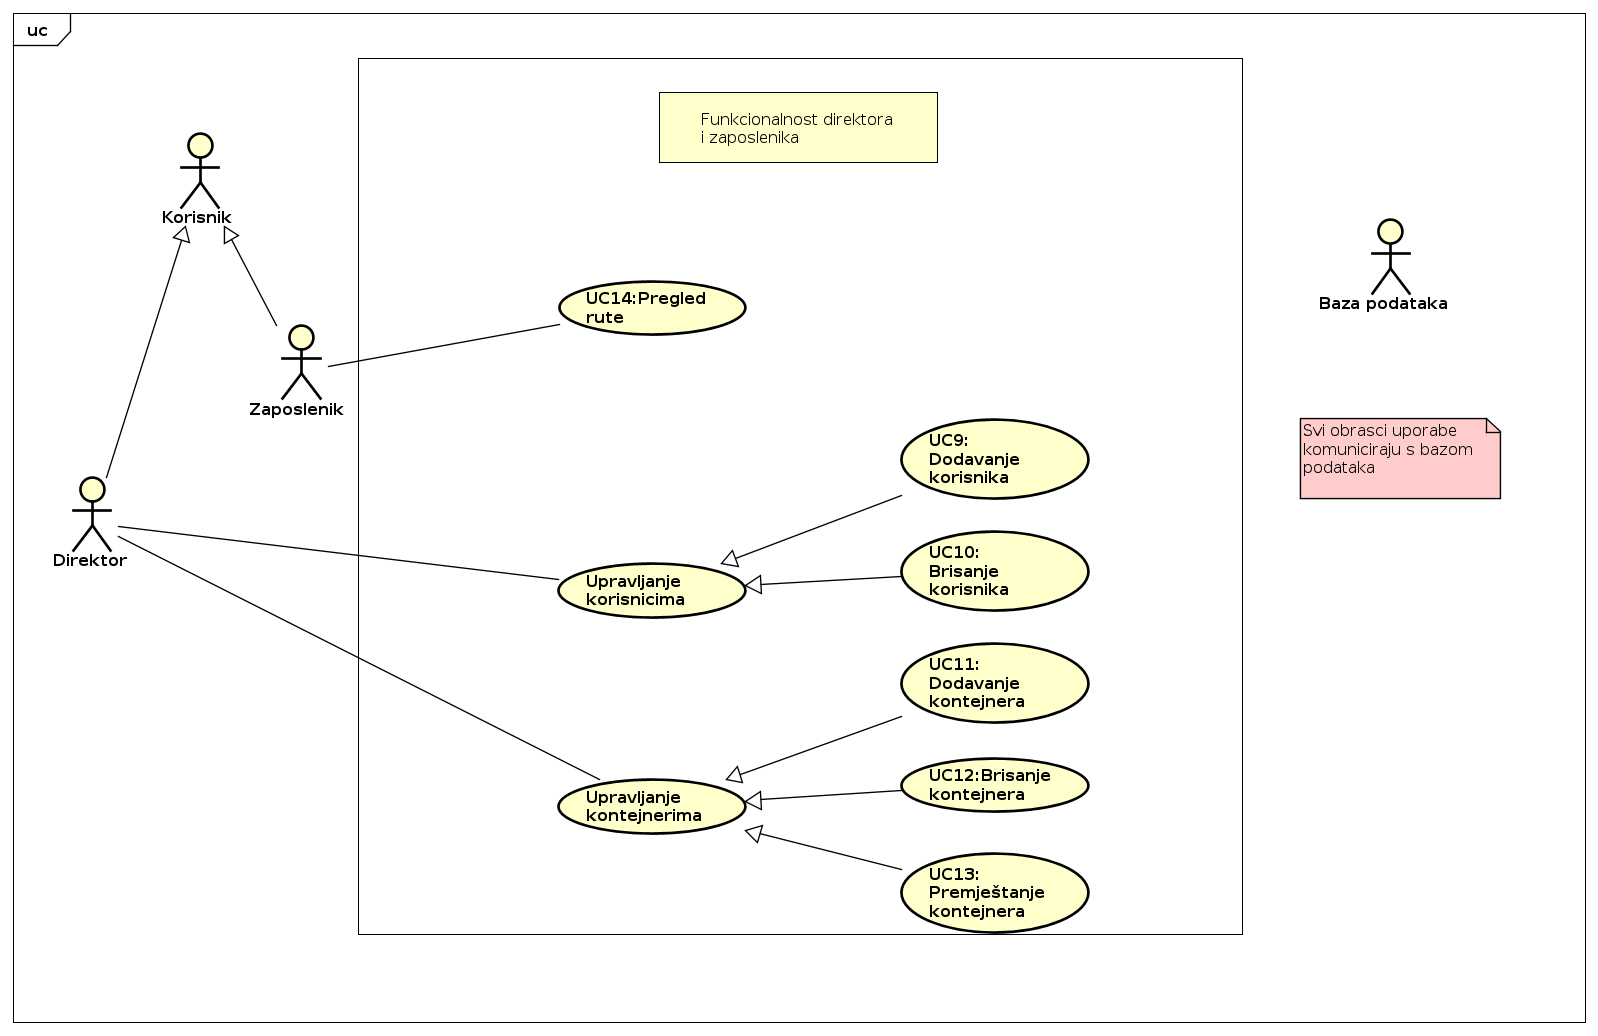
\includegraphics[width=1.0\linewidth]{slike/Funkcionalnost_direktora_i_zaposlenika.png}
                    \caption{Dijagram obrazaca uporabe, funkcionalnost direktora i zaposlenika}
                    \label{fig:Funkcionalnost direktora i zaposlenika}
            \end{figure}
            
            \clearpage
            
			\eject		

			\subsection{Sekvencijski dijagrami}

			\textbf{\textit{dio 1. revizije}}\\
			
			\textit{Nacrtati sekvencijske dijagrame koji modeliraju najvažnije dijelove sustava (max. 4 dijagrama). Ukoliko postoji nedoumica oko odabira, razjasniti s asistentom. Uz svaki dijagram napisati detaljni opis dijagrama.}
			\eject

			\section{Ostali zahtjevi}

			\begin{packed_item}
				\item Sustav treba biti izveden kao responzivna web aplikacija prilagođena mobilnim uređajima, te se prikladno skalirati za ekrane računala
				\item Sustav treba omogućiti rad više korisnika u stvarnom vremenu
				\item Pogreške pri izvođenju se ne smiju direktno prikazivati korisniku
				\item Sustav treba provjeravati ispravnost unesenih podataka, te ne smije dopustiti korisniku da unese podatke koji bi narušili funkcionalnost sustava
				\item Korisničko sučelje sustava mora biti na hrvatskom jeziku, te podržavati hrvatsku abecedu pri unosu i prikazu podataka
				\item Korisničko sučelje mora biti intuitivno i jednostavno za korištenje
				\item Korisniku treba omogućiti pronalazak kontejnera u manje od 10 akcija
				\item Učitavanje stranice ne smije trajati duže od nekoliko sekundi
				\\
				\item Korisničko ime i email adresa korisnika moraju biti jedinstveni
				\item Lozinke se ne smiju spremati u bazu podataka kao nešifrirani tekst \engl{plaintext}, nego moraju biti šifrirane algoritmom raspršivanja
				\item Nakon registracije ili promjene email adrese, potrebno je potvrditi vlasništvo email adrese
				\item Email obavijesti se ne smiju slati na nepotvrđene email adrese.
			\end{packed_item}
